\pagebreak
\section{Question 2}
	
	\subsection{Obtaining Obstacle Location from Laser Data}
	
	First we start by taking the data output from question one, which consisted of the robot ${x-y}$ coordinates in the world coordinate system, as well as the velocity and turn rate for that particular timestamp, for each timestamp that occurs in the Velocity observation data, the Compass data and the GPS data. \newline Similar to the way question one works, we combine this data with the Laser observation data by comparing timestamps, using the Prediction Stage equation to estimate the robots {${x-y}$ coordinates at the time that the laser data was generated. Combining the robots ${x-y}$ world coordinates with the relative position of the obstacles obtained from the Laser data. \newline
				\lstinputlisting{./code/q2/q2_obtain_obstacles.m}
	For initial tests to attempt to identify obstacles, any range reading from the Laser data that was less than eight (the maximum range of the sensor) was considered an obstacle. It was intended to apply filters to this data once the Occupancy Grid had been generated. Until then, raw data would be used.\newline
	
	
%	\begin{figure}[position = here]
%		\begin{centering}
%			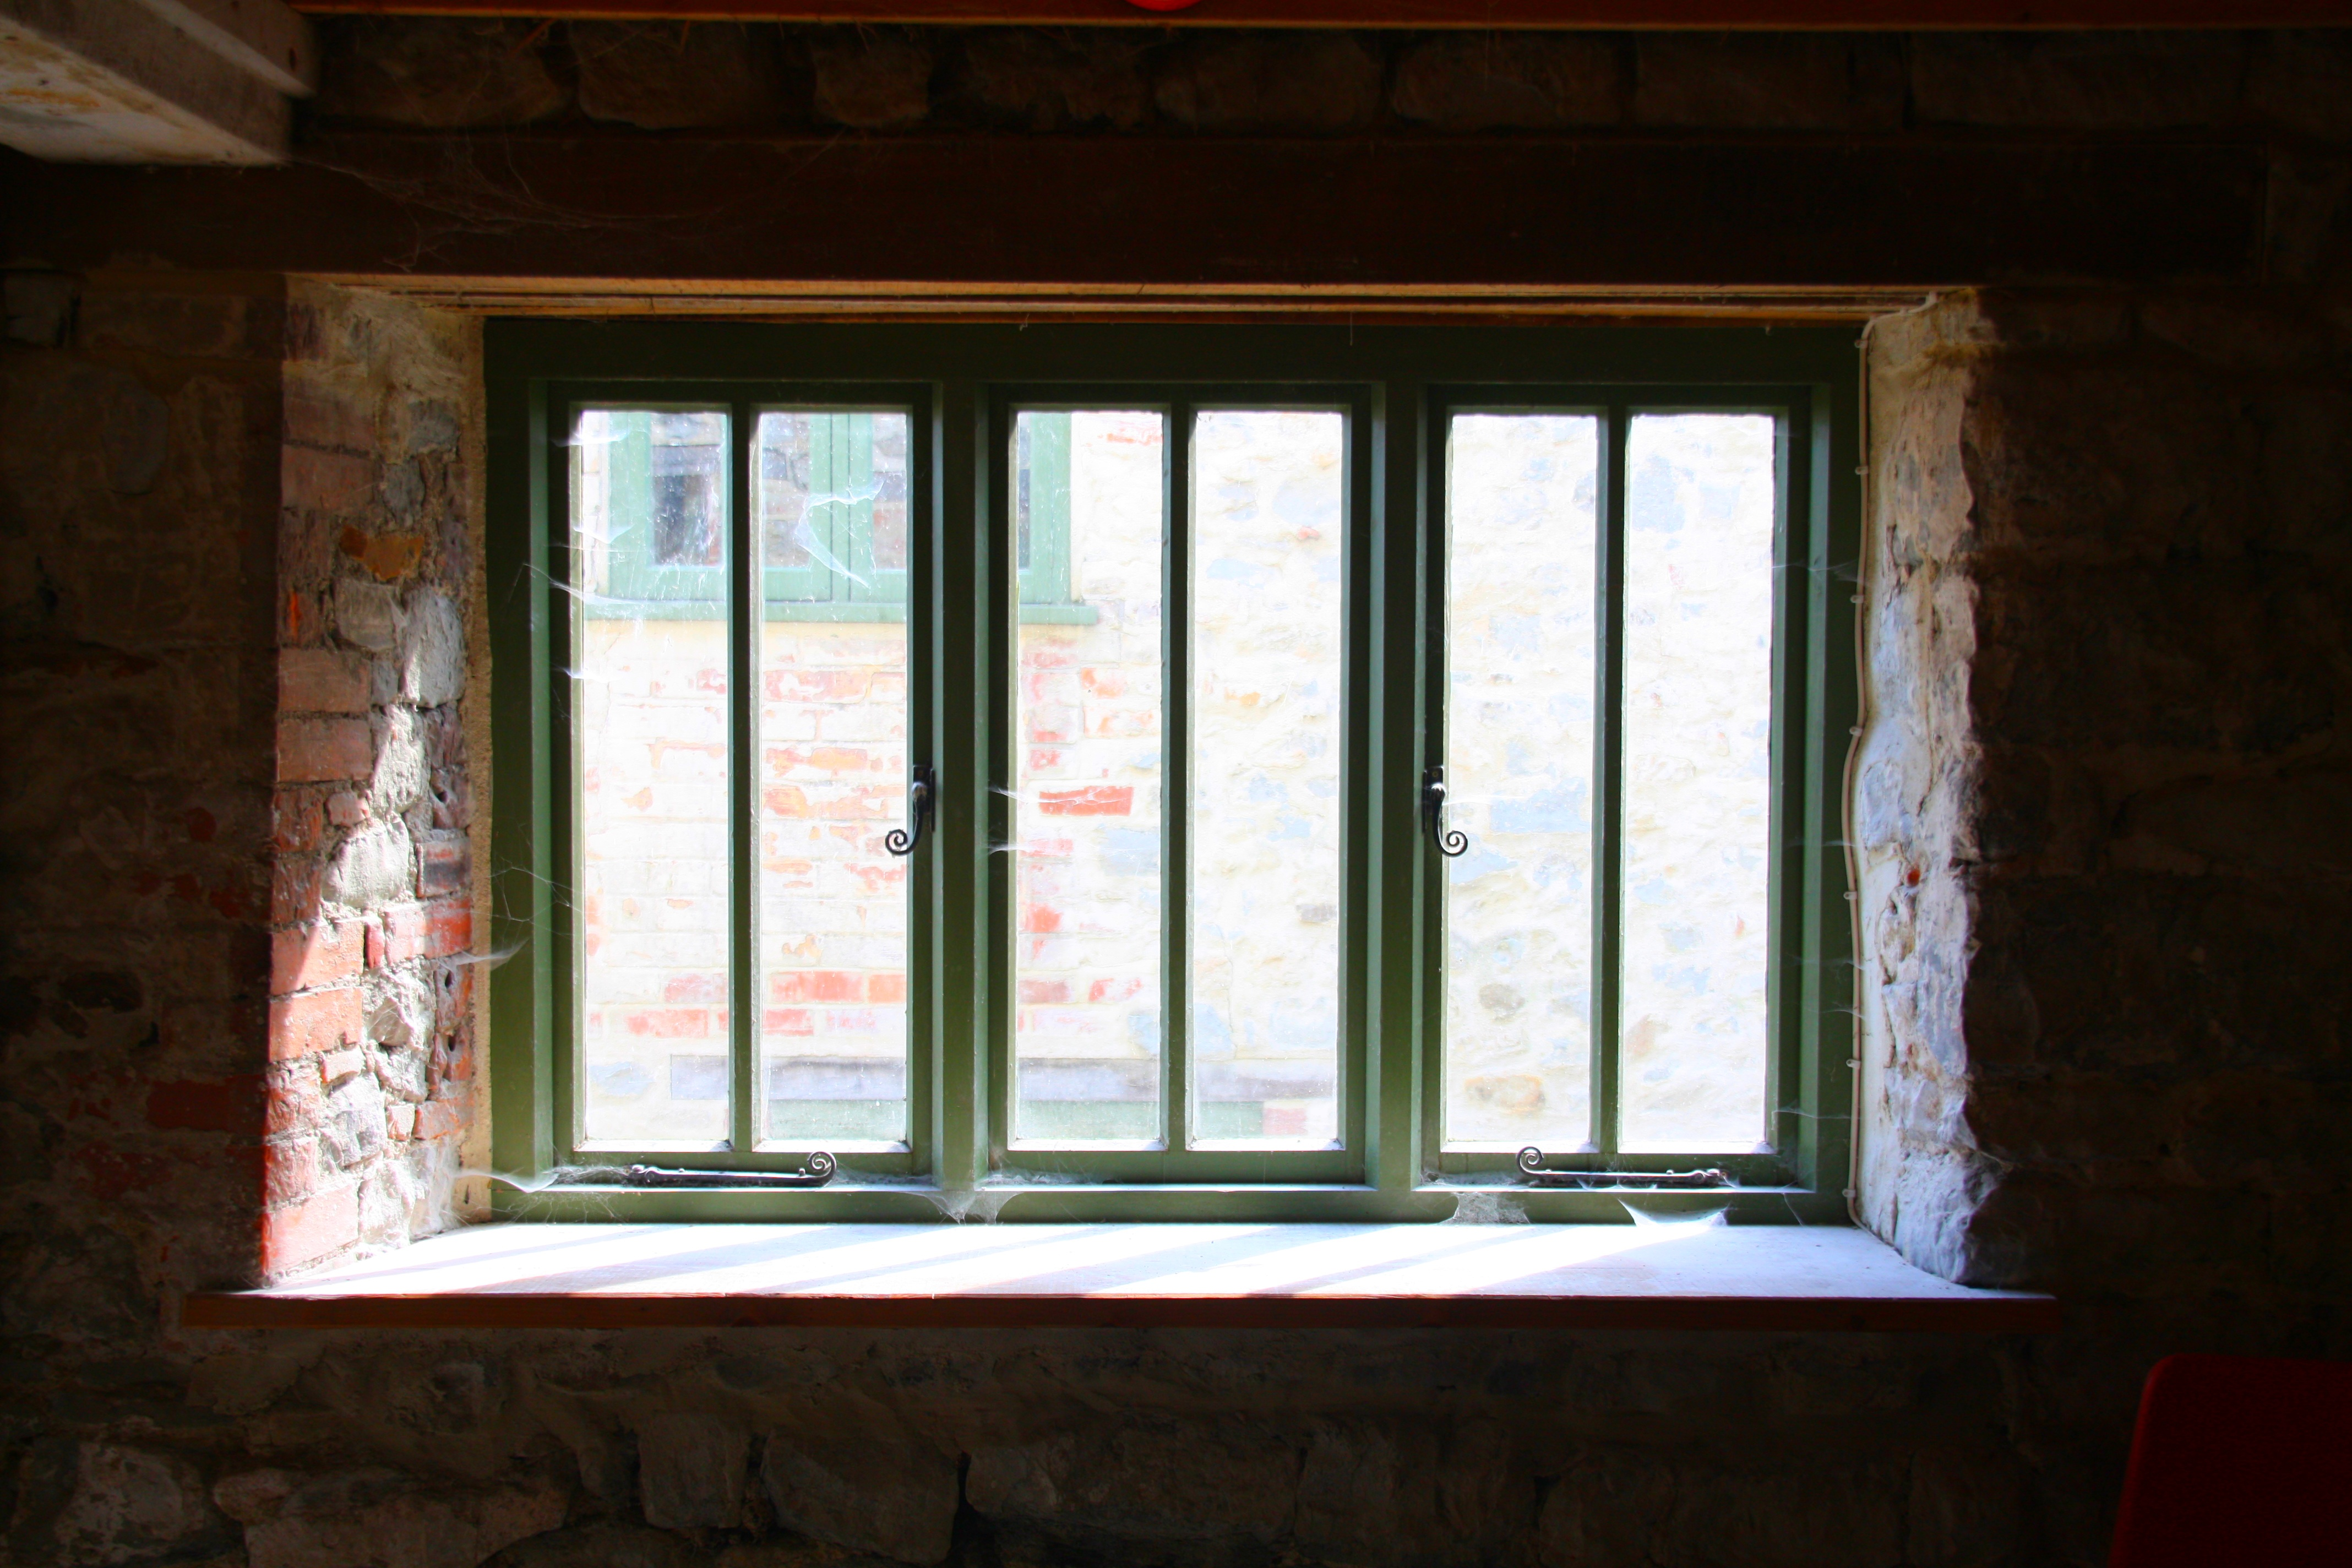
\includegraphics[scale=0.05]{wallWindow}\\
%			\caption[\textit{RPYAxes}]{}
%		\end{centering}
%	\end{figure}
%	\newline
	
	
	\subsection{Generate Occupancy Grid}
	To generate the Occupance Grid, we took the Data set of the X-Y coordinates of all 'Obstacles' detected, and determined the difference between the minimum and maximum ${x}$ and ${y}$ values deteced. Given a user defined size for the occupancy grid, we could then determine the ${x-y}$ range that corresponded to a grid location. Then for every Obstacle ${x-y}$ coordinate we could determine the grid location it corresponded to, incrementing the grid value to increase the weighting, which would indicate the likelihood of an obstacle being in that region. Some experimenting with the grid size using the data for the Robot path generated in question one indicated that a grid size of ${200x200}$ would be best, as this resulted in a grid map that, while not extremely sharp, was also not extremely blurred. Ideally, the grid would be vague enough to generalise a position for the obstacles, but not so clear that it simply resulted in a plot of every possible obstacle coordinates. See the figures below:\newline 
	
		\begin{figure}[position = here]
			\begin{centering}
				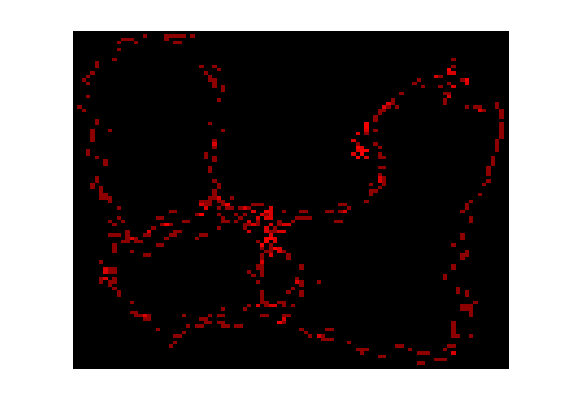
\includegraphics[scale=1]{./images/q2/heatmap_path_100.png}\\
				\caption{Grid size = ${100 \times 100}$}
			\end{centering}
		\end{figure}
		\newline
		
		\begin{figure}[position = here]
			\begin{centering}
				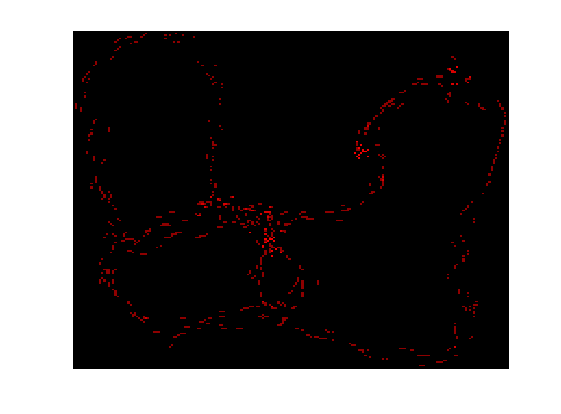
\includegraphics[scale=1]{./images/q2/heatmap_path_200.png}\\
				\caption{Grid size = ${200 \times 200}$}
			\end{centering}
		\end{figure}
		\newline
		
		\begin{figure}[position = here]
			\begin{centering}
				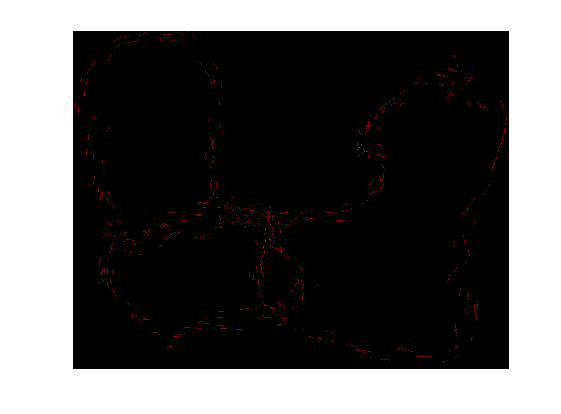
\includegraphics[scale=1]{./images/q2/heatmap_path_500.png}\\
				\caption{Grid size = ${500 \times 500}$}
			\end{centering}
		\end{figure}
		\newline
		
		\pagebreak
	\subsection{Results}
		

\newline